\documentclass[10pt,a4paper]{report}
\usepackage[utf8]{inputenc}
\usepackage{amsmath}
\usepackage{amsfonts}
\usepackage{amssymb}
\usepackage{graphicx}
\usepackage{color}
\usepackage{hyperref}

\hypersetup{
    colorlinks=true,
    linkcolor=blue,
    filecolor=magenta,      
    urlcolor=cyan,
    pdftitle={Overleaf Example},
    pdfpagemode=FullScreen,
    }

\listfiles

\begin{document}
{\LARGE \textbf{Resumen}}

\begin{center}
\begin{tabular}{|c|c|c|c|c|}
\hline
Id (link) & Precio & Tamaño & Puntuación & Dirección \\\hline\hline
%% INSERTAR LINEAS
\end{tabular}
\end{center}


%% REPORTE DE CADA CASA
\newpage
\hypertarget{casa92058112}{}
\begin{center}
\begin{large}
\href{https://www.idealista.com/inmueble/92058112}{\textbf{92058112}}\\[10px]
\end{large}
Direccion\\
Barrio\\
Distrito\\
\end{center}
{\large 123456€ por 789 $m^2$ = \color{blue} \textbf{4321}}\\[20px]
Esta kelly es la puta hostia!
\begin{figure}[htbp]
%% IMAGENES DE LA CASA
% 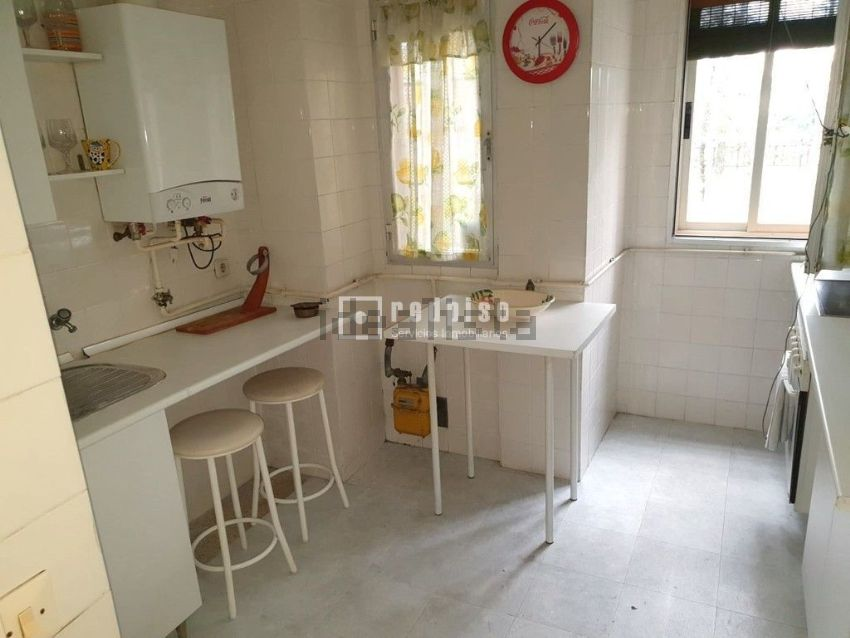
\includegraphics[width=0.5\textwidth]{arfima/92058112/92058112-001.jpg}
\caption{selected images (92058112)}
\end{figure}

%% FIN DEL REPORTE DE CADA CASA


\end{document}